\chapter{Code structure}

\section{Introduction}

The original WAQBANK code was developed in MATLAB.
For \dfastbe we have selected Python because

\begin{itemize}
\item The Python environment is available for free contrary to MATLAB.
\item Python is a popular coding language for software developers and domain specialists and users alike, and it's therefore easier for development cycle.
\item The use of NumPy should enable use to code the algorithm with a similar performance as MATLAB.
\item Python allows to create redistributable binaries that are similar or smaller in size than MATLAB (including the MATLAB Compiler Runtime environment).
\item Python combines well with the open source nature of this software and other developments in the Delft3D / D-HYDRO environment.
\end{itemize}

The software uses a number of Python modules for specific functionality.
Most importantly the code builds on

\begin{itemize}
\item \keyw{netCDF4} for reading and writing netCDF files.
\item \keyw{NumPy} for the numerical computations using arrays.
\item \keyw{PyQt5} for the graphical user interface.
\item \keyw{Shapely} for common geometric operations.
\item \keyw{geopandas} for some geospatial operations and IO of geospatial files.
\item \keyw{matplotlib} for creating graphs.
\end{itemize}

The various file formats used and written by \dfastbe are described in \autoref{Chp:FileFormats}.
The next section describes the subdivision of the code into modules.


\section{Listing of modules}

\dfastbe is subdivided into 9 modules:

\begin{itemize}
\item \keyw{\_\_init\_\_.py} module level file containing mainly the version number.
\item \keyw{\_\_main\_\_.py} module level file containing argument parsing and call to \keyw{dfastbe.cmd.run()}.
\item \keyw{cmd.py} containing the main run routine.
\item \keyw{gui.py} for the graphical user interface.
\item \keyw{batch.py} for the command line interface (batch mode).
\item \keyw{io.py} for all file handling: reading of input and configuration files as well as writing of results files.
\item \keyw{kernel.py} for all scientific steps of the algorithm.
\item \keyw{support.py} for various (mostly geometric) steps of the algorithm.
\item \keyw{plotting.py} for the creation of the figures.
\end{itemize}

All files (except for \keyw{\_\_init\_\_.py}) are addressed individually in the following subsections.


\subsection{main function \keyw{cmd.py} and command line interface \keyw{\_\_main\_\_.py}}

The parsing of the command line arguments occurs in \keyw{\_\_main\_\_.py} and the file \keyw{cmd.py} implements the main routine.
The \keyw{\_\_main\_\_} module depends on the \keyw{cmd} module which in turn depends on the \keyw{batch}, \keyw{gui} and \keyw{io} modules.
Depending on the command line arguments \dfastbe will run in one of three modes:

\begin{enumerate}
\item Bank line detection mode (\keyw{banklines}).
It takes the analysis configuration file as input, obtains the relevant data from the \dflowfm result file, performs the bank detection analysis and writes the bank line file(s) and a reference figure.
\item Bank erosion mode (\keyw{bankerosion}).
It takes the analysis configuration file as input, reads the bank line file(s), obtains the relevant data from the \dflowfm result files, performs the bank erosion analysis and writes a number of files with bank erosion data and figures.
\item Graphical user interface (\keyw{gui}).
It allows the user to interactively specify the parameters needed for the analysis.
The settings can be saved for later batch processing or a batch analysis can be started immediately.
\end{enumerate}

The following command line options are supported for this purpose

\begin{tabular}{l|l|p{8cm}}
short & long & description \\ \hline
\keyw{-h} & \keyw{-{}-help} & show help text and exit \\
 & \keyw{-{}-language} & language selection: \keyw{NL} or \keyw{UK} (default: \keyw{UK}) \\
 & \keyw{-{}-mode} & run mode \keyw{banklines}, \keyw{bankerosion} or \keyw{gui} (default: \keyw{gui}) \\
 & \keyw{-{}-config} & name of analysis configuration file (default: \keyw{dfastbe.cfg}) \\
\end{tabular}

These files contain one routine each:

\begin{itemize}
\item \keyw{parse\_arguments} parses the command line arguments and returns those values (included in \keyw{\_\_main\_\_.py}).
\item \keyw{run} initializes the language support and starts the appropriate run mode (included in \keyw{cmd.py}).
\end{itemize}

and the main code that triggers the parsing of the command line arguments (via \keyw{parse\_arguments}) and executes \keyw{run} based on those settings.


\subsection{graphical user interface \keyw{gui.py}}

This module implements the graphical user interface version of \dfastbe.
It can be used to generate and edit the analysis configuration files for both the bank line detection and bank erosion steps.
This module depends on the \keyw{batch} and \keyw{io} modules.

\begin{figure}
\center
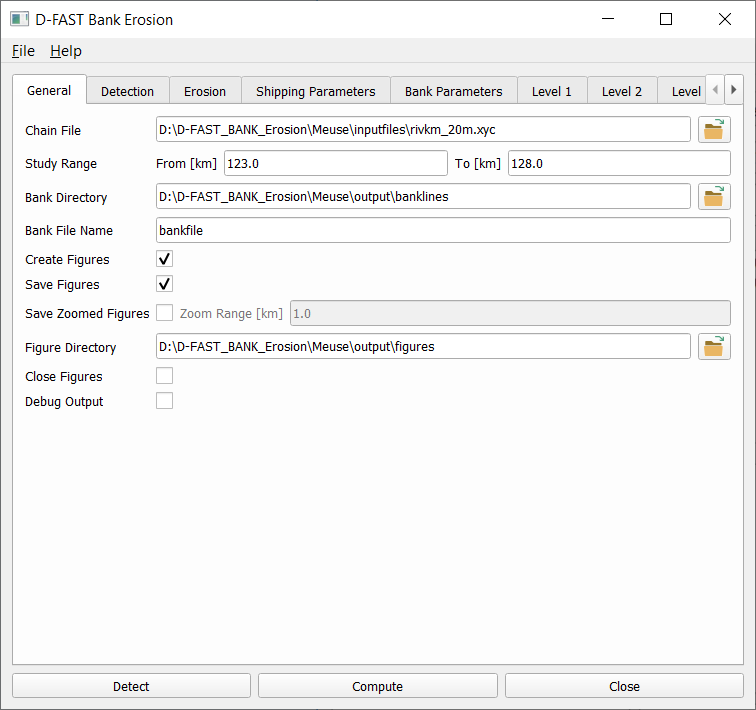
\includegraphics[width=\textwidth]{figures/gui1.png}
\caption{Example of the main dialog}
\end{figure}

This module contains the following routines:

\begin{itemize}
\item \keyw{gui\_text} queries the global dictionary of texts for a single string in the GUI.
\item \keyw{create\_dialog} to create the graphical user interface.
\item \keyw{createMenus} adds the menus to the menubar.
\item \keyw{addGeneralTab} creates the tab for the general settings.
\item \keyw{addDetectTab} creates the tab for the bank line detection settings.
\item \keyw{addErosionTab} creates the tab for the main bank erosion settings.
\item \keyw{addShippingTab} creates the tab for the general shipping settings.
\item \keyw{shipTypes} returns the tuple of ship types.
\item \keyw{addBankTab} creates the tab for the general bank properties.
\item \keyw{bankStrengthSwitch} implements the dialog settings depending on the bank strength specification method.
\item \keyw{validator} creates validators.
\item \keyw{activate\_dialog} hands over control to the user interface.
\item \keyw{generalParLayout} adds a line of controls for editing a general parameter.
\item \keyw{addOpenFileRow} adds a line of controls for selecting a file or folder in a form layout.
\item \keyw{getIcon} opens the icon file relative to the location of the program.
\item \keyw{openFileLayout} creates a standard layout with a file or folder edit field and selection button.
\item \keyw{addRemoveEditLayout} creates a standard layout with list control and add, edit and remove buttons.
\item \keyw{updatePlotting} updates the plotting flags.
\item \keyw{addAnItem} implements the actions for the add item button.
\item \keyw{setDialogSize} sets the width and height of a dialog and position it centered relative to the main window.
\item \keyw{editASearchLine} creates an edit dialog for the search lines list.
\item \keyw{editADischarge} create an edit dialog for simulation file and weighing.
\item \keyw{close\_edit} implements a generic close function for edit dialogs.
\item \keyw{editAnItem} implements the actions for the edit item button.
\item \keyw{removeAnItem} implements the actions for the remove item button.
\item \keyw{updateTabKeys} renumber simulation tab $i$ to tab $i-1$.
\item \keyw{selectFile} selects a file or directory via a selection dialog.
\item \keyw{selectFolder} selects a folder via a folder selection dialog.
\item \keyw{run\_detection} runs the bank line detection based on settings in the GUI.
\item \keyw{run\_erosion} runs the D-FAST Bank Erosion analysis based on settings in the GUI.
\item \keyw{close\_dialog} support function to close the dialog and end the program.
\item \keyw{menu\_load\_configuration} selects and loads a configuration file.
\item \keyw{load\_configuration} opens a configuration file and update the GUI accordingly.
\item \keyw{addTabForLevel} creates the tab for the settings associated with simulation $i$.
\item \keyw{optionalParLayout} adds a line of controls for editing an optional parameter.
\item \keyw{typeUpdatePar} implements the dialog setting switching for both general and optional parameters.
\item \keyw{setParam} updates the dialog for a general parameter based on configuration file.
\item \keyw{setOptParam} updates the dialog for an optional parameter based on configuration file.
\item \keyw{menu\_save\_configuration} asks for a configuration file name and save GUI selection to that file.
\item \keyw{get\_configuration} extracts a configuration from the GUI.
\item \keyw{showError} displays an error message box with specified string.
\item \keyw{menu\_about\_self} and \keyw{menu\_about\_qt} callback functions to show About boxes.
\item \keyw{menu\_open\_manual} callback function to open the user manual
\item \keyw{show\_error} support function to show an error dialog.
\item \keyw{main} starts the user interface using default settings or optional configuration.
\end{itemize}


\subsection{batch mode \keyw{batch.py}}

This module implements the main routines of 'banklines' and 'bankerosion' algorithms of \dfastbe, as well as a number of helper routines.
This module depends on the \keyw{io}, \keyw{kernel}, \keyw{support} and \keyw{plotting} modules.

\begin{enumerate}
\item Bank line detection mode ('banklines').
This is the first step of the algorithm that detects the location of the banks based on a representative \dflowfm simulation and an initial hint regarding the banks of interest.
\item Bank erosion estimation mode ('bankerosion').
This is the second step of the algorithm which uses the bank location and various \dflowfm simulation results as input and estimates the bank erosion rates and volumes and indicates the resulting retreated bank lines.
\end{enumerate}

This module contains the following routines:

\begin{itemize}
\item \keyw{banklines} implements the first part of the algorithm, namely the bank line detection.
\item \keyw{banklines\_core} runs the bank line detection analysis for a specified configuration.
\item \keyw{bankerosion} implements the second part of the algorithm, namely the bank erosion estimation.
\item \keyw{bankerosion\_core} runs the bank erosion analysis for a specified configuration.

\item \keyw{adjust\_filenames} converts all paths to relative to current working directory.
\item \keyw{get\_bbox} derives the bounding box from a line.
\item \keyw{derive\_topology\_arrays} derives the secondary topology arrays from the face\_node\_connectivity.
\item \keyw{debug\_file} writes a text file for debugging.
\item \keyw{timedlogger} prints selected text to screen with timing information.
\item \keyw{timer} tracks time and prints timing information
\item \keyw{config\_to\_absolute\_paths} converts a configuration object to contain absolute paths (for editing).
\item \keyw{config\_to\_relative\_paths} converts a configuration object to contain relative paths (for saving).
\item \keyw{parameter\_absolute\_path} converts a parameter value to contain an absolute path.
\item \keyw{parameter\_relative\_path} converts a parameter value to contain a relative path.
\end{itemize}


\subsection{general input/output \keyw{io.py}}

The \keyw{io.py} module contains all file handling routines for reading configuration files, processing netCDF input and output files, and functions to support various input and output formats.
This module does not depend on any other \dfastbe module.

This module contains the following routines:

\begin{itemize}
\item \keyw{load\_program\_texts} fills a global dictionary of dialog texts by reading the dialog text configuration file
\item \keyw{log\_text} obtains one text from the global dictionary of dialog texts and writes it to screen or file
\item \keyw{get\_filename} obtains a file name from the global dictionary of dialog texts
\item \keyw{get\_text} obtain one text from the global dictionary of dialog texts

\item \keyw{write\_config} support function to write a nicely formatted analysis configuration file.

\item \keyw{read\_fm\_map} for reading data fields from the \dflowfm map-file
\item \keyw{get\_mesh\_and\_facedim\_names} for obtaining the name of the 2D mesh and the name of the corresponding face dimension
\item \keyw{copy\_ugrid} for copying UGRID mesh information from the \dflowfm map-file to the spatial output file
\item \keyw{copy\_var} support function for copying an individual netCDF variable from netCDF file to another
\item \keyw{ugrid\_add} for adding a single cell centred variable to a netCDF file containing UGRID mesh data

\item \keyw{read\_waqua\_xyz} for reading the xyz-files containing data exported from the WAQUA model (legacy function)
\item \keyw{write\_simona\_box} for writing a SIMONA BOX-file (legacy function)

\item \keyw{absolute\_path} converts a relative path into an absolute path given a reference path
\item \keyw{relative\_path} converts an absolute path into a path relative to a given reference path

\item \keyw{read\_xyc} read line geometry files and chainage file.
\item \keyw{write\_km\_eroded\_volumes} write a text file with eroded volume data binned per kilometre.

\item \keyw{read\_config} reads an analysis configuration file -- this routine just reads the file, it does not perform any checking of the parameters.
\item \keyw{upgrade\_config} upgrade the configuration data structure to version 1.0 format.
\item \keyw{movepar} move a parameter from one group/keyword to another.

\item \keyw{config\_get\_xykm} get chainage line and clip it to the range of interest.
\item \keyw{clip\_chainage\_path} clip a chainage line to the relevant reach.
\item \keyw{config\_get\_search\_lines} get $N$ search lines for the bank locations.
\item \keyw{config\_get\_bank\_lines} get the bank lines from the detection step.
\item \keyw{config\_get\_bank\_search\_distances} get the search distance per bank line from the analysis settings.
\item \keyw{config\_get\_simfile} get the name of the simulation file from the analysis settings.
\item \keyw{config\_get\_range} get a range (as minimum and maximum value) from the analysis configuration file.
\item \keyw{config\_get\_str}, \keyw{config\_get\_float}, \keyw{config\_get\_int}, \keyw{config\_get\_bool} get string, float, integer and boolean value from the analysis configuration file.
\item \keyw{config\_get\_parameter} get a parameter value per bank node (either by expanding a constant value or by reading one or more parameter files).
\item \keyw{get\_kmval} read a parameter file, check its contents and return arrays of chainages and values.
\item \keyw{read\_simdata} for reading all relevant data from the \dflowfm map-file.
\item \keyw{get\_progloc} returns the absolute path for the program location
\end{itemize}


\subsection{core algorithm \keyw{kernel.py}}

The \keyw{kernel.py} module contains all routines for that perform the mathematical processing steps of the algorithm.
This module does not depend on any other \dfastbe module.

This module contains the following routines:

\begin{itemize}
\item \keyw{comp\_erosion\_eq} computes the equilibrium erosion distance per bank line segment given the reference flow conditions.
\item \keyw{comp\_erosion} computes the erosion distance per bank line segment given a single flow condition.
\item \keyw{edge\_mean} averages the parameter values from the bank line nodes to the bank line segments.
\item \keyw{comp\_hw\_ship\_at\_bank} compute the ship induced wave height at the beginning of the fore shore.
\item \keyw{get\_km\_bins} expand the chainage range and step size to a list of chainage bin boundary values.
\item \keyw{get\_km\_eroded\_volume} accumulate the eroded volumes per chainage bin.
\end{itemize}


\subsection{(geometric) support routines \keyw{support.py}}

The \keyw{support.py} module contains all support routines that are not related to IO or core algorithm formulations.
Most of these routines include geometric processing.
This module does not depend on any other \dfastbe module except for the definition of the SimulationObject for type checking.

This module contains the following routines:

\begin{itemize}
\item \keyw{project\_km\_on\_line} transfer the chainage information from the chainage line to another line.
\item \keyw{on\_right\_side} determine whether a line is to the left or right of a reference line.
\item \keyw{xykm\_bin} resample a georeferenced chainage line to bin boundaries.
\item \keyw{intersect\_line\_mesh} intersect a line with a mesh to arrive at line segments uniquely linked to mesh faces.
\item \keyw{get\_slices} intersect a (bank) line with an unstructured mesh and return the intersection coordinates and mesh face indices.
\item \keyw{get\_slices\_core} intersect a (bank) line with an unstructured mesh and return the intersection coordinates and mesh face indices.
\item \keyw{get\_slices\_ab} get the relative locations a and b at which a segment intersects/slices a number of edges.
\item \keyw{map\_line\_mesh} determine for each node of a line in which cell (face) of the mesh it's located.
\item \keyw{move\_line} shift a line of a variable distance sideways (positive shift away from centre line).
\item \keyw{move\_line\_right} shift a line of a variable distance sideways (positive shift to the right).
\item \keyw{add\_point} add the x,y-coordinates of a point to an array of x,y-coordinates if it differs from the last point.
\item \keyw{clip\_sort\_connect\_bank\_lines} connect the bank line segments to bank lines and clip to the area of interest.
\item \keyw{clip\_search\_lines} clip ta list of lines to the envelope of certain size surrounding a reference line.
\item \keyw{convert\_search\_lines\_to\_bank\_polygons} construct a series of polygons surrounding the bank search lines.
\item \keyw{clip\_simdata} clip simulation data to region within a specified distance from a line.
\item \keyw{get\_banklines} detect all possible bank line segments based on simulation data.
\item \keyw{poly\_to\_line} detect the bank line segments inside an individual face of arbitrary (convex) polygonal shape.
\item \keyw{tri\_to\_line} detect the bank line segments inside an individual triangle.
\end{itemize}


\subsection{plotting \keyw{plotting.py}}

The \keyw{plotting.py} module contains all routines related to creating figures for \dfastbe (intermediate) results.
This module does not depend on any other \dfastbe module, but most of the routines in this module depend on matplotlib.

This module contains the following routines:

\begin{itemize}
\item \keyw{savefig} save a single figure to file.
\item \keyw{setsize} set the size of a figure.
\item \keyw{set\_bbox} specify the bounding limits of an axes object.
\item \keyw{chainage\_markers} add markers indicating the river chainage to a plot.
\item \keyw{plot\_mesh} add a mesh to a plot.
\item \keyw{plot\_mesh\_patches} add a collection of patches to the plot one for every face of the mesh.

\item \keyw{plot\_detect1} create the bank line detection plot.

\item \keyw{plot1\_waterdepth\_and\_banklines} create the bank erosion plot with water depths and initial bank lines.
\item \keyw{plot2\_eroded\_distance\_and\_equilibrium} create the bank erosion plot with predicted bank line shift and equilibrium bank line.
\item \keyw{plot3\_eroded\_volume\_subdivided\_1} create the bank erosion plot with total eroded volume subdivided per discharge level.
\item \keyw{plot3\_eroded\_volume\_subdivided\_2} create the bank erosion plot with total eroded volume subdivided per bank.
\item \keyw{plot4\_eroded\_volume\_eq} create the bank erosion plot with equilibrium eroded volume.
\item \keyw{plot5series\_waterlevels\_per\_bank} create the bank erosion plots with water levels, bank height and bank protection height along each bank.
\item \keyw{plot6series\_velocity\_per\_bank} create the bank erosion plots with velocities and critical velocities along each bank.
\item \keyw{plot7\_banktype} create the bank erosion plot with colour-coded bank types.
\item \keyw{plot8\_eroded\_distance} create the bank erosion plot with total and equilibrium eroded distance.
\item \keyw{get\_colors} obtain N colors from the specified colormap.
\end{itemize}
